\documentclass[11pt]{article}
\usepackage[margin=1in]{geometry}
\usepackage{amsmath,amssymb,amsthm,mathtools}
\usepackage{graphicx}
\usepackage{microtype}
\usepackage[colorlinks=true,linkcolor=blue,urlcolor=blue,citecolor=blue]{hyperref}

\newtheorem{theorem}{Theorem}
\newcommand{\D}{\mathbb D}
\newcommand{\B}{\mathcal B}
\newcommand{\C}{\mathbb C}
\newcommand{\Aut}{\operatorname{Aut}}

\title{The constants do not split invariantly in the Bloch space}
\author{Candidate full negative answer to a question in arXiv:2211.06055}
\date{11 August 2026}

\begin{document}
\maketitle

\noindent\fbox{\parbox{0.94\linewidth}{\textbf{Status: candidate full proof, likely valid.}
The constant functions have no algebraic complement in the classical Bloch
space that is invariant under the M\"obius composition action.  Invariance
under one explicit hyperbolic automorphism already gives a contradiction.}}

\section{Source question}

Let
\[
 \B(\D)=\left\{f\in\operatorname{Hol}(\D):
 \beta(f):=\sup_{z\in\D}(1-|z|^2)|f'(z)|<\infty\right\}
\]
with its usual seminorm, whose nullspace is the one-dimensional space
$\C\mathbf 1$ of constants.  Calzi's survey asks whether one can find a
$\widetilde U_0$-invariant algebraic complement of $\C\mathbf 1$ in
$\B(\D)$, and records that the existence of such spaces was unknown
\cite[p.~3, footnote~1]{Calzi}.

\begin{figure}[ht]
\centering
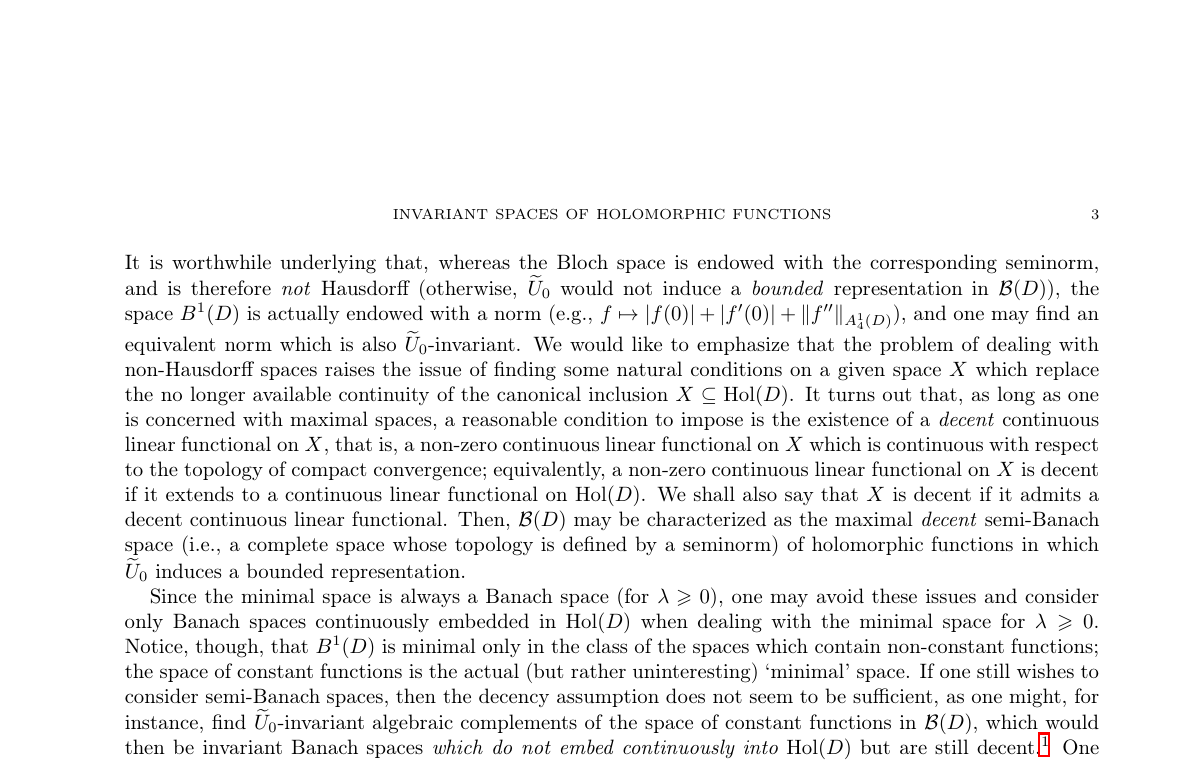
\includegraphics[width=\linewidth]{figures/source_question_body.png}
\vspace{0.25em}

\includegraphics[width=\linewidth]{figures/source_question_footnote.png}
\caption{The complement question and its ``we do not know'' footnote on page 3
of the source.}
\end{figure}

Here $U_0$ is the composition action (up to the harmless choice of inverse),
so that $U_0(\psi)f=f\circ\psi^{-1}$ for $\psi\in\Aut(\D)$.

\clearpage

\section{Proof intuition}
Conjugating one hyperbolic disk automorphism by the Cayley map turns it into
multiplication by $2$ on the right half-plane.  The normalized logarithm of
the Cayley map is a Bloch function satisfying the Abel equation
$h\circ\phi-h=1$.  An invariant algebraic complement would induce a
projection onto constants that commutes with composition by $\phi$; that
projection must annihilate the coboundary on the left but fix the constant
on the right, an immediate contradiction.

\section{Negative answer}

\begin{theorem}
There is no vector subspace $Y\subseteq\B(\D)$ such that
\[
 \B(\D)=\C\mathbf 1\oplus Y
\]
algebraically and $f\circ\psi\in Y$ for every $f\in Y$ and every
$\psi\in\Aut(\D)$.  In fact, no such $Y$ exists even if invariance is
required only under the cyclic group generated by
\[
 \phi(z)=\frac{3z+1}{z+3}.
\]
\end{theorem}

\begin{proof}
Consider the Cayley map from the disk to the right half-plane,
\[
 C(z)=\frac{1+z}{1-z}.
\]
Multiplication by $2$ is an automorphism of the right half-plane, and
\[
 \phi=C^{-1}\circ(2C),\qquad
 \phi(z)=\frac{3z+1}{z+3},\qquad C(\phi(z))=2C(z).
\]
Let $\operatorname{Log}$ be the principal logarithm.  Since $C(\D)$ is the
right half-plane, the function
\[
 h(z)=\frac{\operatorname{Log}C(z)}{\log 2}
\]
is holomorphic on $\D$.  Positive real scaling does not change the argument,
so the principal branch gives the exact Abel equation
\begin{equation}\label{eq:Abel}
 h(\phi(z))-h(z)=1\qquad(z\in\D).
\end{equation}

The function $h$ belongs to the Bloch space.  Indeed,
\[
 h'(z)=\frac{2}{(1-z^2)\log 2},
\]
while
\[
 |1-z^2|^2-(1-|z|^2)^2=4(\operatorname{Im}z)^2\ge0.
\]
Consequently
\[
 (1-|z|^2)|h'(z)|\le \frac{2}{\log 2}
 \qquad(z\in\D).
\]

Suppose now that an invariant algebraic complement $Y$ exists, and let
$P:\B(\D)\to\C\mathbf1$ be the algebraic projection along $Y$.  Constants
are fixed by composition, and invariance under both $\phi$ and $\phi^{-1}$
gives $f\circ\phi\in Y$ exactly when $f\in Y$.  Hence
\[
 P(f\circ\phi)=P(f)\qquad(f\in\B(\D)).
\]
Applying $P$ to \eqref{eq:Abel} yields
\[
 0=P(h\circ\phi)-P(h)=P(\mathbf1)=\mathbf1,
\]
a contradiction.
\end{proof}

\section{Strength and scope}

The proof is algebraic.  It does not assume that $Y$ is closed, that the
projection $P$ is continuous, or that an orbit map is measurable.  It also
uses only one hyperbolic disk automorphism.  More generally, any
composition-invariant vector space of holomorphic functions which contains
$\mathbf1$ and the displayed Abel function $h$ has no complement of the
constants invariant under $\phi$.

This settles the specific existence question on page 3 of the source.  It does
not settle the separate question later in the survey asking whether every
$\lambda$-invariant semi-Banach space is ultradecent.

Bounded searches of the local run indexes and the web on 11 August 2026 used
the arXiv identifier, the exact complement language, Bloch constants,
M\"obius invariance, and Abel equations.  They found no later answer to the
footnote and no matching nonsplitting proof.  Novelty confidence is moderate:
the construction is elementary and the Abel function itself is classical.

\begin{thebibliography}{1}
\bibitem{Calzi}
M.~Calzi, \emph{A Survey on Invariant Spaces of Holomorphic Functions on
Symmetric Domains}, arXiv:2211.06055v3 (2022),
\url{https://arxiv.org/abs/2211.06055}.
\end{thebibliography}

\end{document}
